\chapter{Desenvolvimento}%
    \label{chp:Desenvolvimento}
	
	\section{O OpenServer}
	
    	Visando oferecer mais liberdade e flexibilidade para o usuário, no que diz respeito à programação da malha de controle adicional e ao dispositivo que irá executá-la, foi desenvolvido um programa chamado OpenServer, isto é, o servidor do sistema Open. Este, tem também o objetivo de trazer mais segurança para a controladora do robô do laboratório do CEFET-MG em Divinópolis durante a execução de malhas de controle experimentais. 
    	
    	O OpenServer é executado no LPC e utiliza a biblioteca \ac{eORL} para intermediar a comunicação entre a controladora robô e o LPC, ou seja, utiliza a estrutura do sistema Open fornecida pela fabricante. Ele oferece uma \textit{API} (Interface de Programação de Aplicativo, em tradução livre) baseada em rede \ac{TCPIP} para se comunicar com um programa cliente em um terceiro dispositivo. Este programa cliente tem o papel de enviar as referências das juntas do robô para o OpenSever, que por sua vez tem que repassar estas referências para a controladora do robô. Ao mesmo tempo, o OpenSever tem o papel de receber da controladora os dados sensoriais do robô (posição angular das juntas, por exemplo) e repassar para o programa cliente. Como a comunicação entre controladora e o LPC pode ocorrer a uma taxa diferente da comunicação do LPC com o terceiro dispositivo, o OpenServer tem que conseguir realizar a comunicação de forma assíncrona. 
    	
    	O objetivo é que o programa cliente possa ser escrito em qualquer linguagem de programação que suporte o protocolo \ac{TCPIP} e que possa rodar em qualquer sistema operacional que tenha suporte ao mesmo. E que o dispositivo no qual o programa cliente esteja rodando possa ser de qualquer arquitetura de processador, desta forma, permitindo que até dispositivos móveis como \textit{smartphones} que utilizem a \textit{API} do OpenServer.
        
        Acredita-se que essa abordagem possa reduzir riscos ao equipamento por erro ou imperícia ao ser programada uma malha de controle usando recursos do sistema \textit{Open} fornecidos pelo fabricante. Pois o OpenServer pode ser programado para continuar se comunicando com a controladora, mesmo que a conexão com o programa cliente seja perdida ocasionada por um fechamento inesperado do programa cliente ou um travamento, enquanto que, se este programa estivesse sendo executado no LPC, a comunicação com a controladora seria encerrada bruscamente. Além disso, o OpenServer é capaz de oferecer uma alternativa de \textit{API} mais simples de ser aprendida e utilizada.
	
        A estrutura padrão do sistema fornecida pela empresa fabricante é detalhada na Figura~\ref{conexoes-padrao}, onde: (1) é a conexão elétrica entre Controladora e Manipulador Robótico; (2) representa a conexão \textit{PowerLink} entre \ac{LPC} e controladora; (3) é a conexão entre roteador e controladora; e (4) conexão entre roteador e o \ac{LPC}.
    
        \begin{figure}[ht]
            \centering
            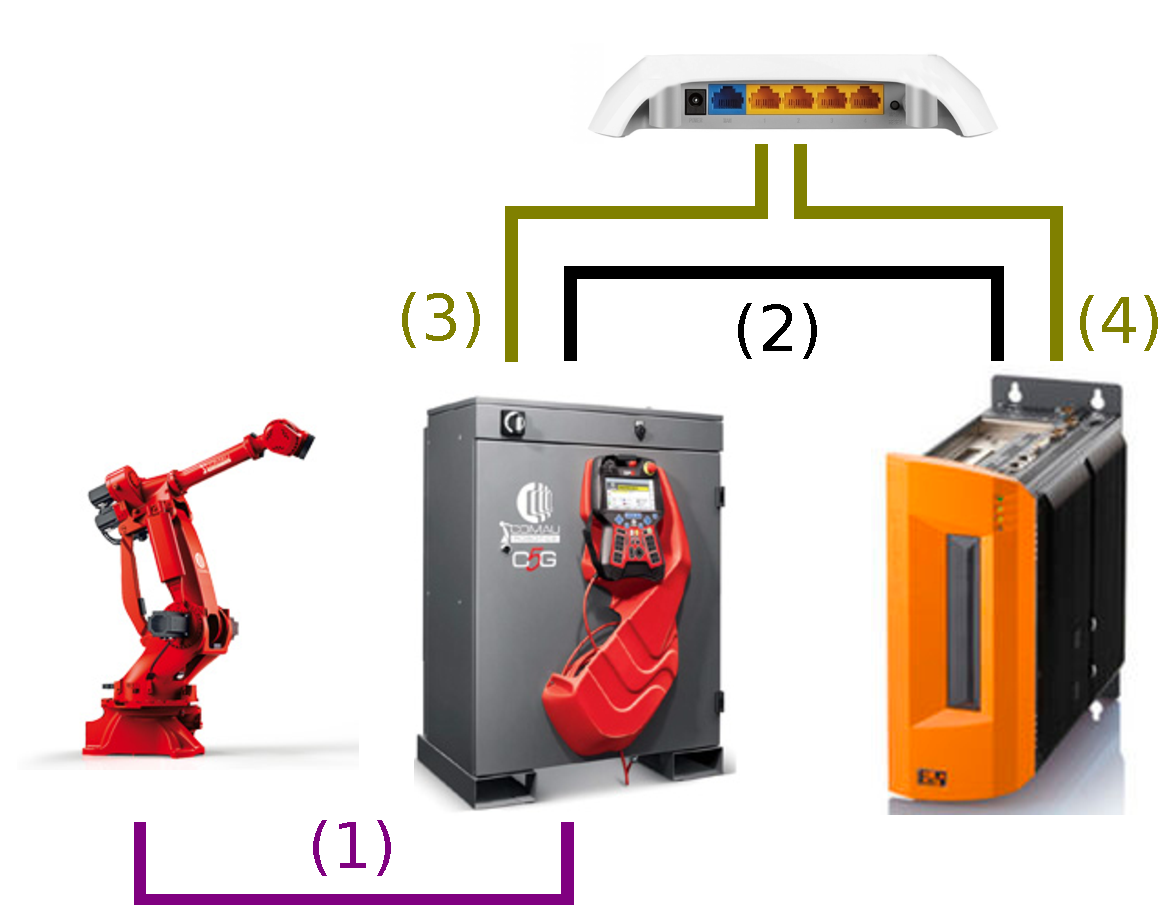
\includegraphics[width=10cm]{imagens/Conexoes/conexoes-padrao.eps}
            \small 
            \centering 
            \caption{Estrutura padrão do sistema C5G Open}
            \label{conexoes-padrao}
        \end{figure}
          
        Como dito anteriormente, o OpenServer foi desenvolvido para utilizar-se a estrutura padrão do sistema fornecida pela empresa fabricante. Logo, foi programado dentro das limitações da plataforma, ou seja, na linguagem C++ usando a biblioteca \ac{eORL} do fabricante do robô, sendo usada a conexão \textit{Ethernet PowerLink} do LPC para fazer a comunicação com a controladora do robô e sendo compilado para o sistema operacional baseado em Linux com arquitetura x86. Além disso, ele usa a rede \textit{Ethernet} convencional do LPC e bibliotecas padrão em C++ disponíveis para o sistema operacional \textit{Linux Mint} para realizar a comunicação via protocolo \ac{TCPIP}. A estrutura desenvolvida para execução do OpenServer passa então a ser conforme é mostrado na Figura~\ref{conexoes-openserver}, onde: (5) representa a conexão entre o roteador e o dispositivo externo, que pode ser feita através de cabeamento ou conexão sem fio; e (6) é a conexão entre roteador e rede institucional.
        
        \begin{figure}[ht]
            \centering
            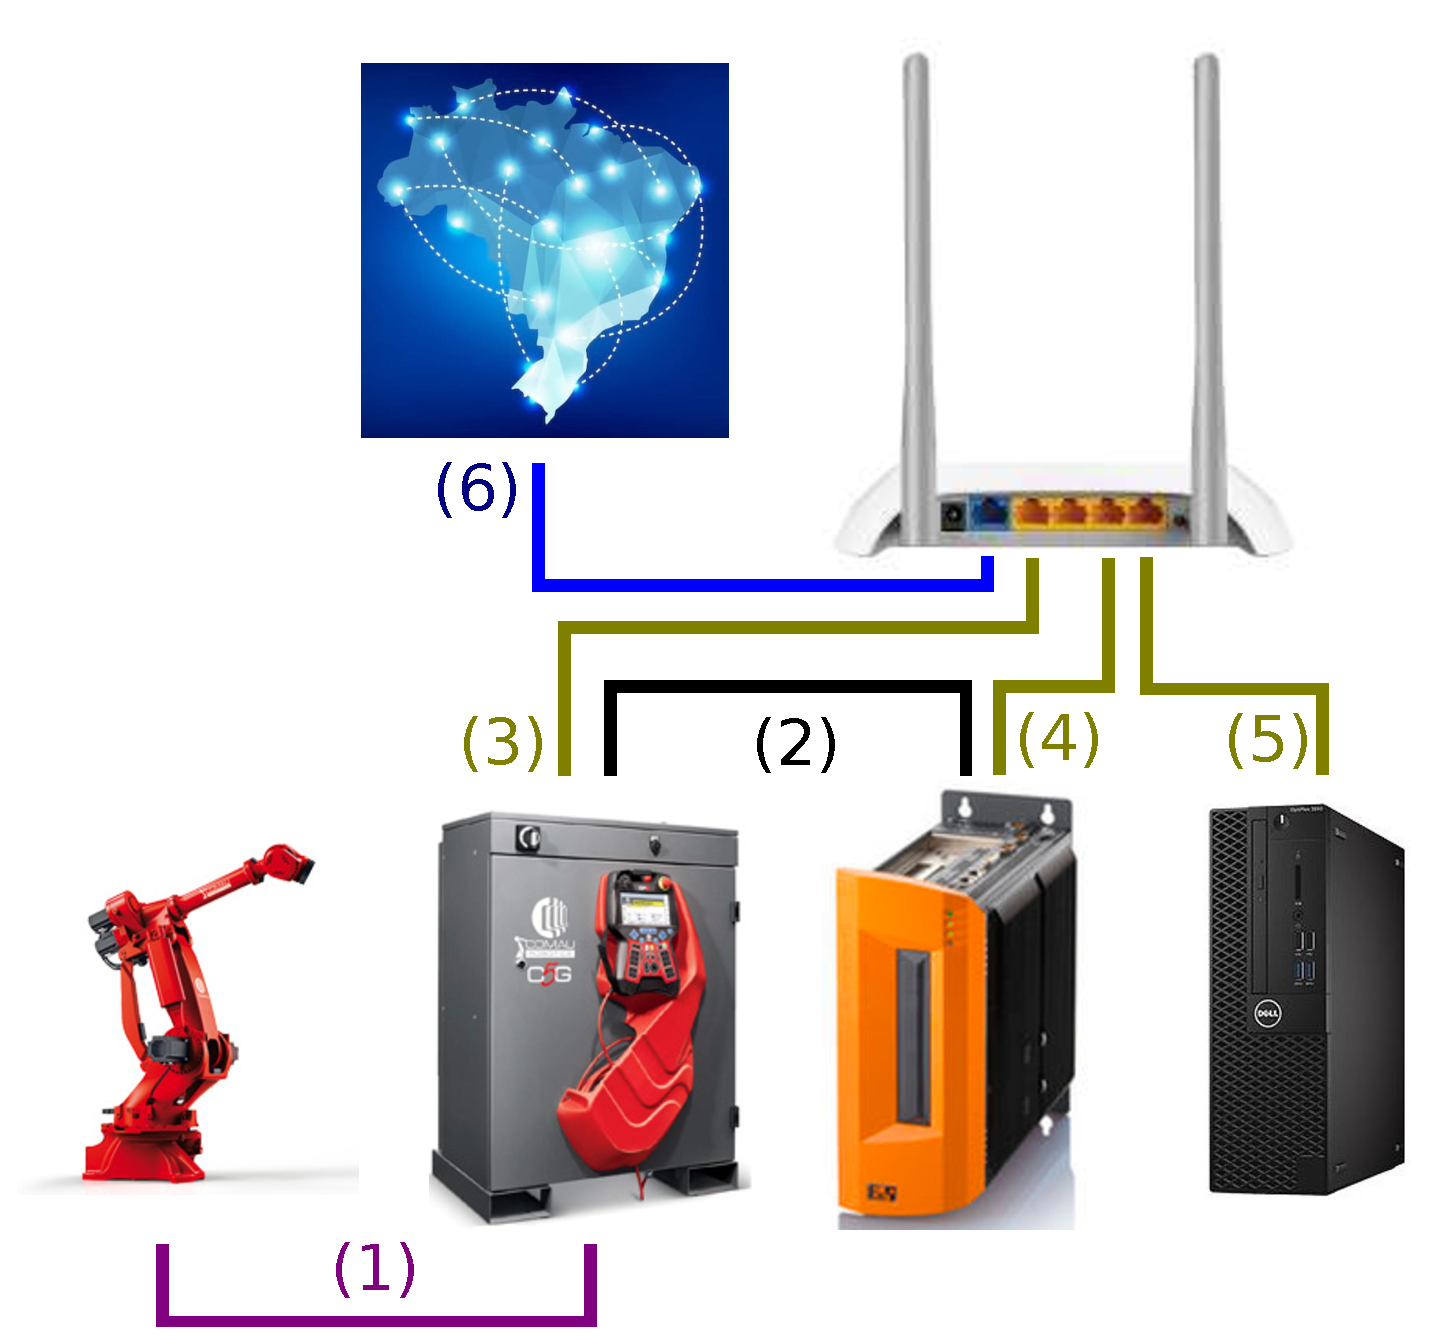
\includegraphics[width=10cm]{imagens/Conexoes/conexoes-openserver.eps}
            \small 
            \centering 
            \caption{Estrutura desenvolvida para execução do OpenServer}
            
            \label{conexoes-openserver}
        \end{figure}
        
        A rede institucional do CEFET-MG oferece acesso à internet. No entanto, as portas do roteador são bloqueadas para acesso externo. Dessa forma, é criada uma rede interna segura onde os programas se comunicarão. Por esta razão, não foram implementadas soluções de criptografia de dados, bem como de autenticação. Isso ocorreu também pelo motivo de ser um ambiente acadêmico, controlado e sem trafego de dados sensíveis. A estrutura real do sistema pode ser visto na Figura~\ref{lab1}. Estão disponíveis também dois computadores conectados à rede interna, que podem ser vistos na Figura~\ref{lab2}, para a execução de programas clientes.
        
        \begin{figure}[ht]
            \centering
            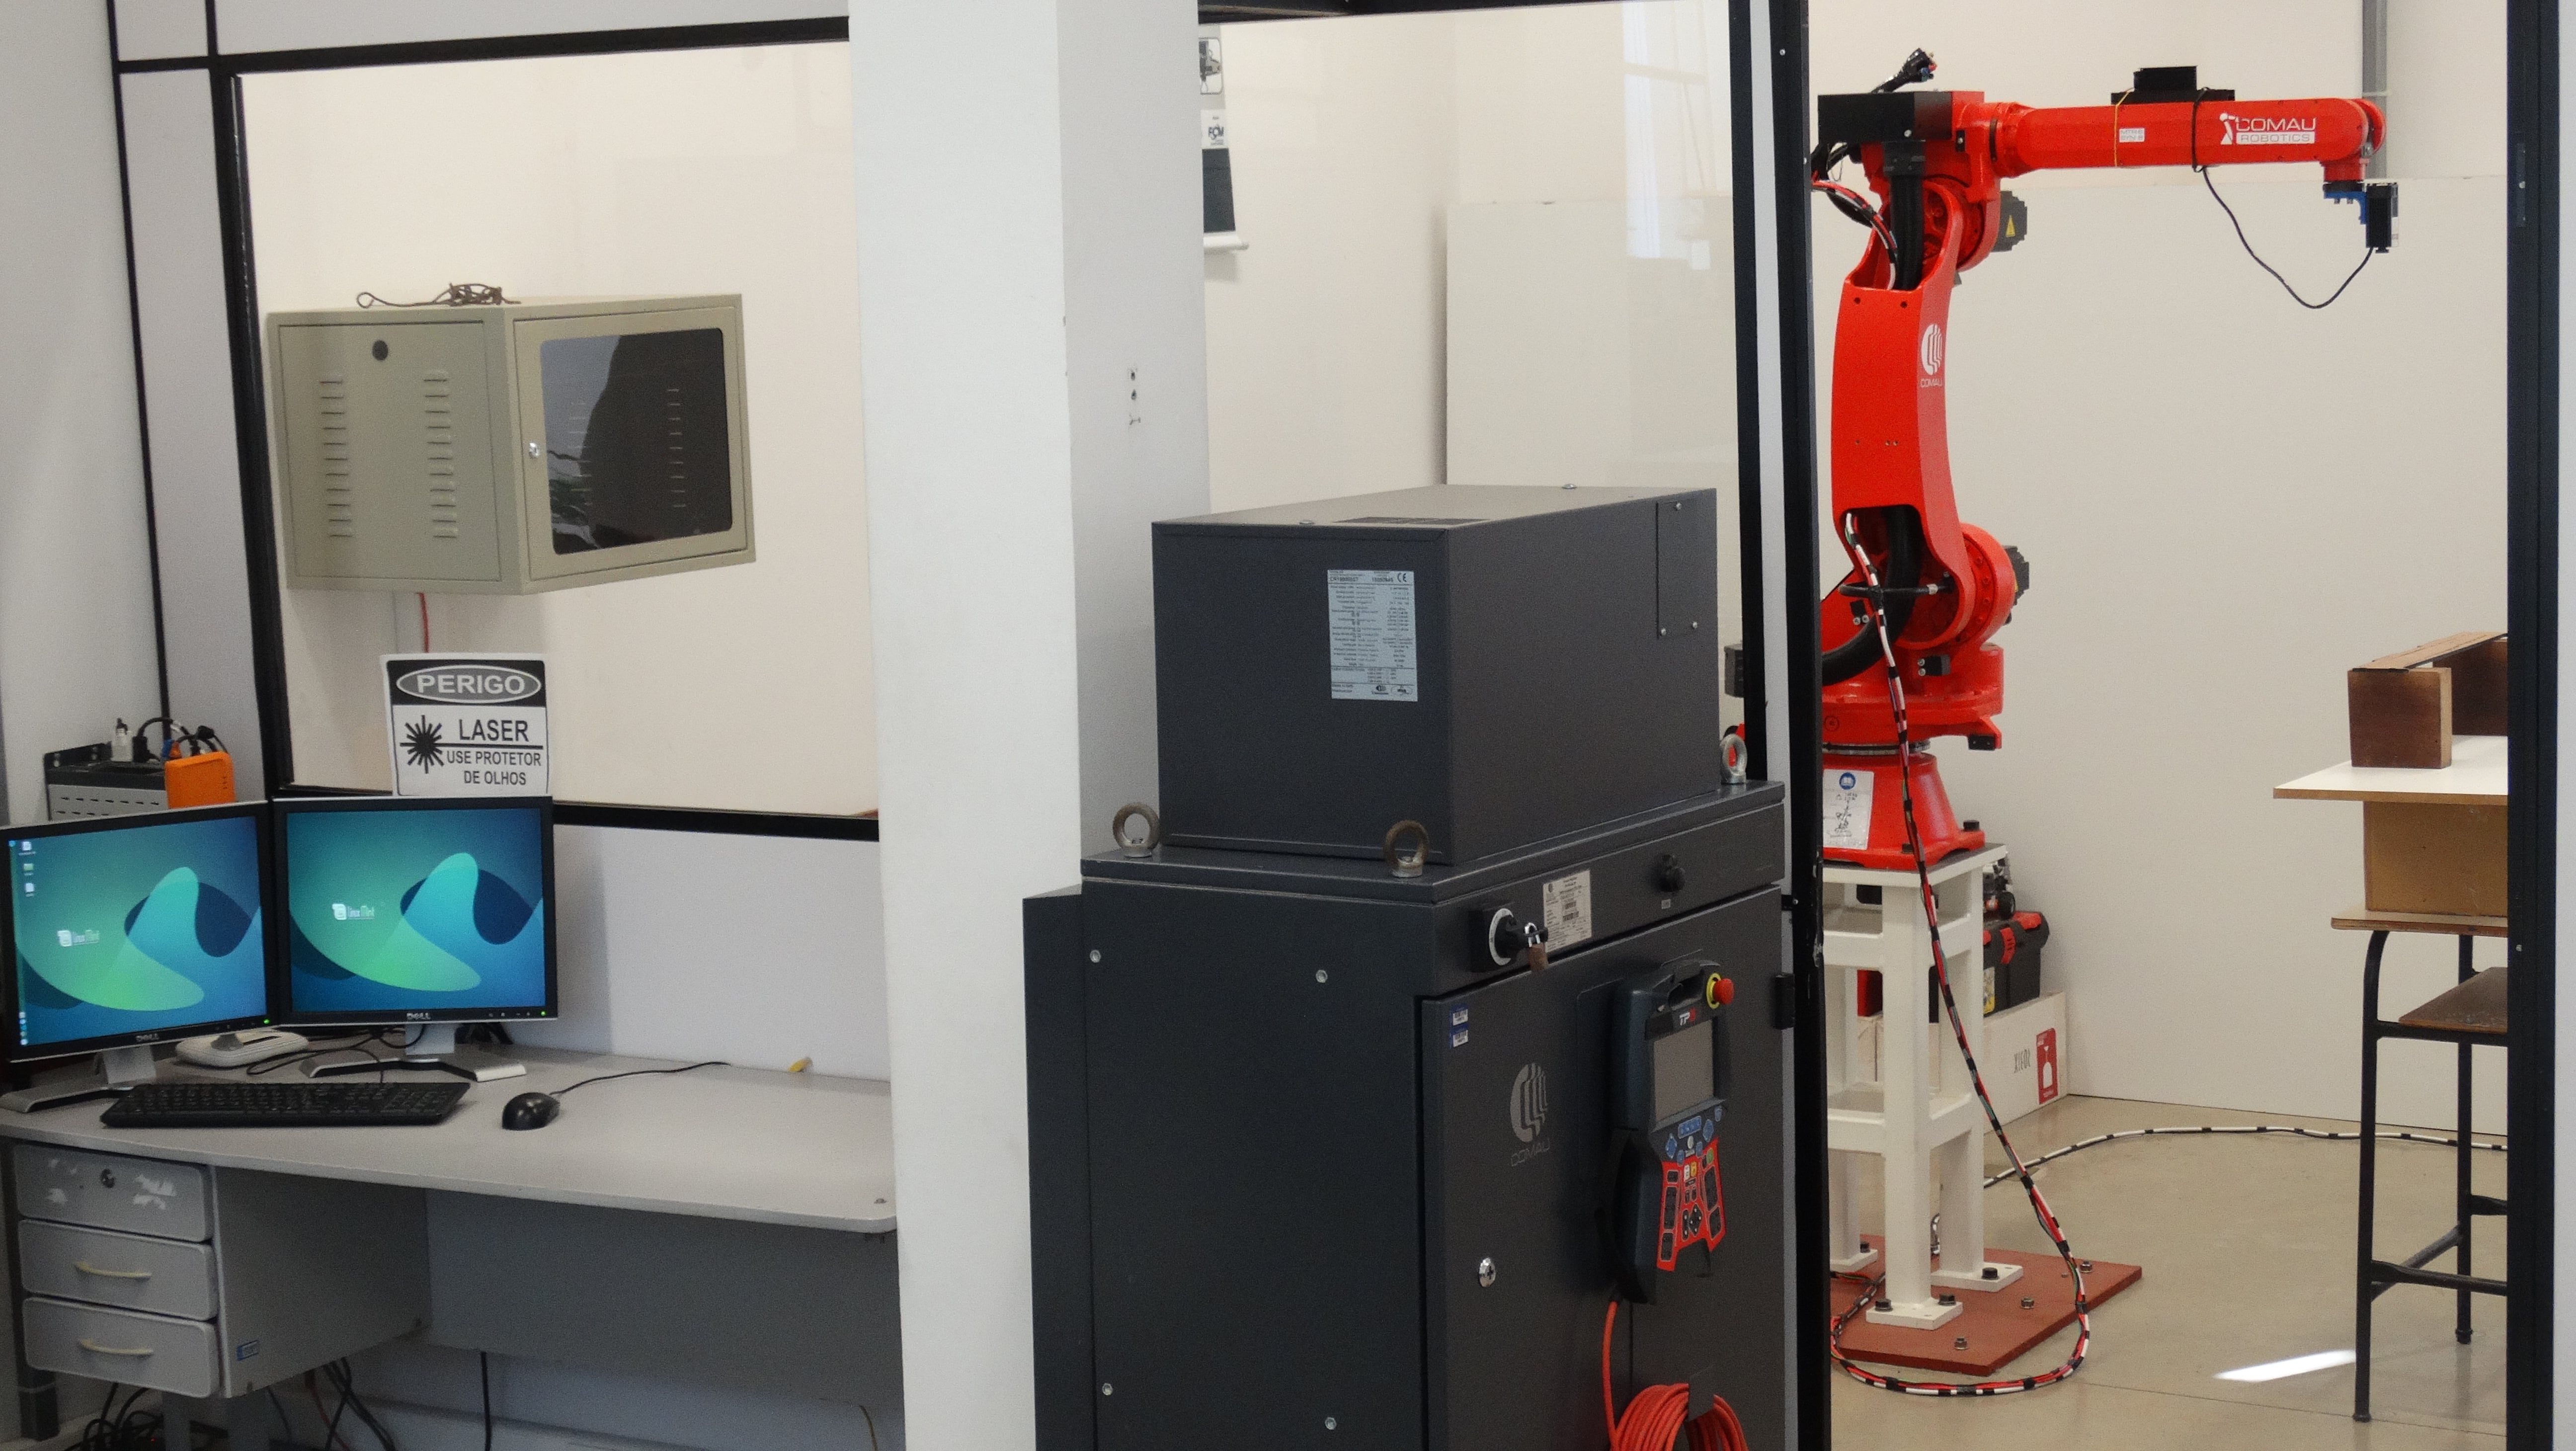
\includegraphics[width=\columnwidth]{imagens/Fotos/estrutura-lab-1.JPG}
            \small 
            \centering 
            \caption{Estrutura do laboratório: robô, controladora e \ac{LPC}}
            \label{lab1}
        \end{figure}
        
        \begin{figure}[ht]
            \centering
            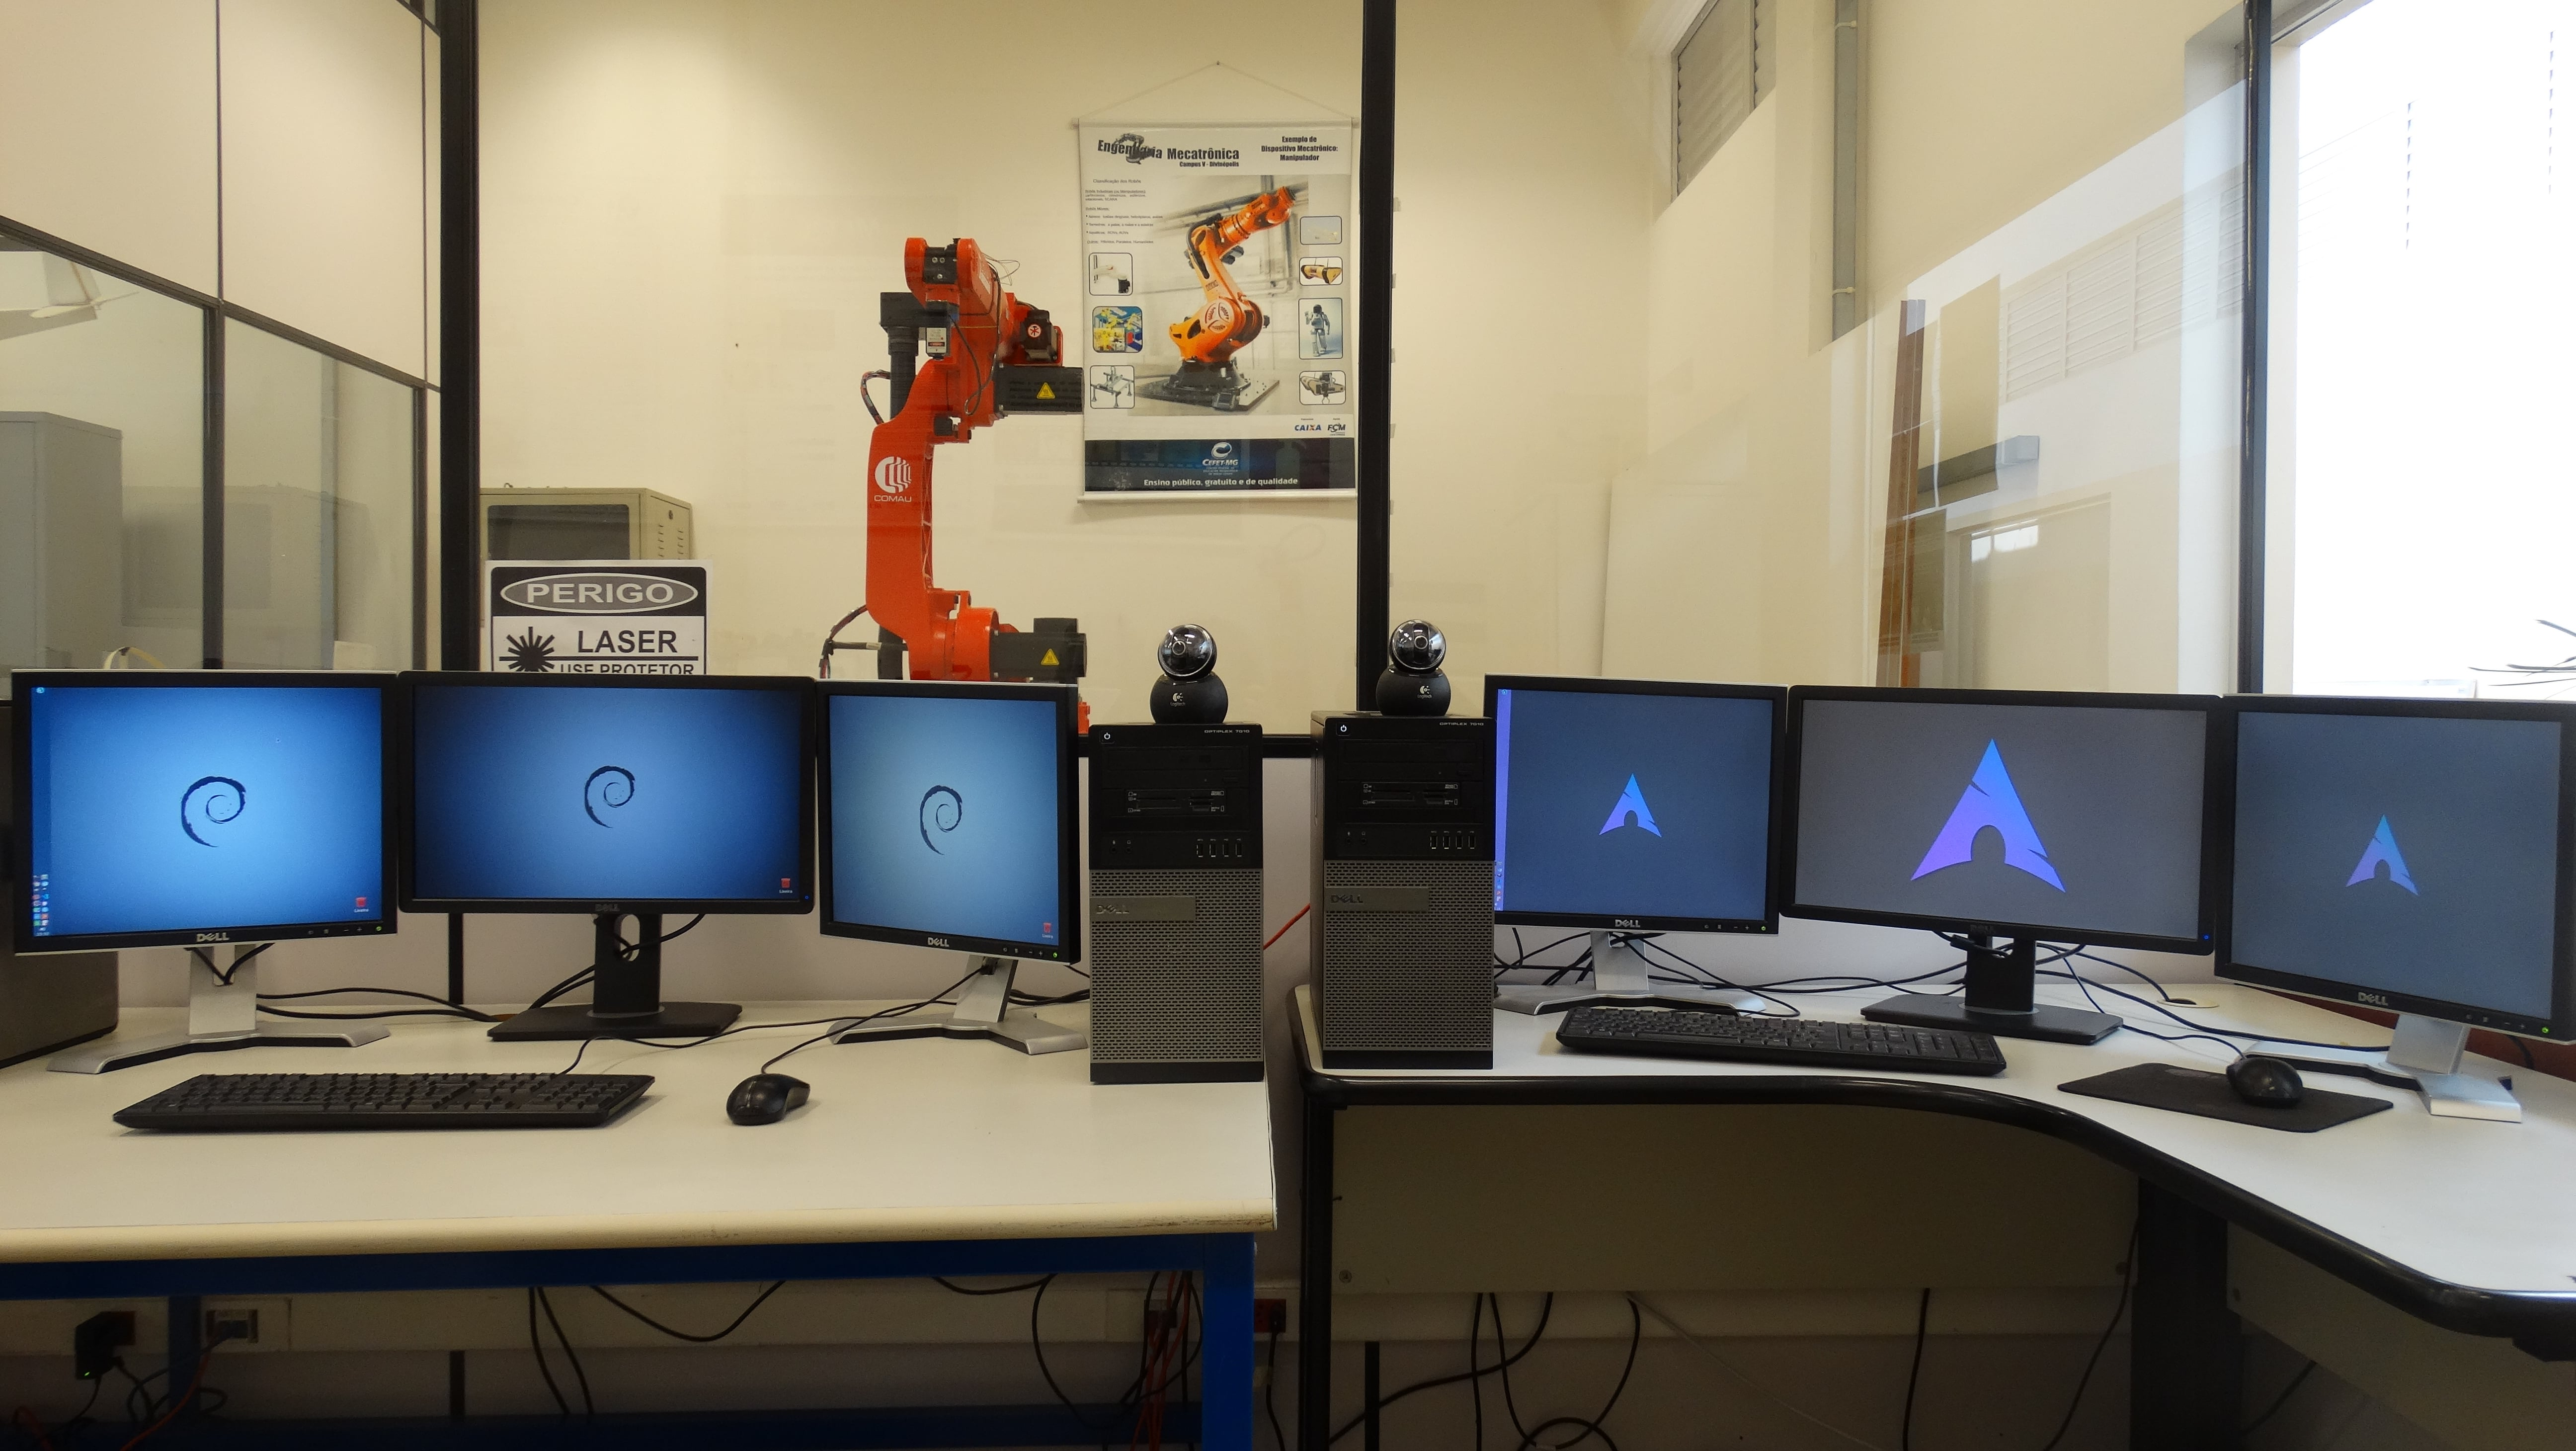
\includegraphics[width=\columnwidth]{imagens/Fotos/estrutura-lab-2.JPG}
            \small 
            \centering 
            \caption{Estrutura do laboratório: computadores onde serão executados os programas clientes}
            \label{lab2}
        \end{figure}
        
        O desenvolvimento desta abordagem torna mais segura a utilização do sistema Open em um ambiente de ensino e pesquisa, pois o único programa que precisará ser executado no \ac{LPC} passa a ser o \textit{OpenSever} em uma versão estável. Já no dispositivo externo serão executados os programas experimentais ou em desenvolvimento, os quais podem travar durante a execução, por exemplo, entre outros acontecimentos que podem gerar uma falha de comunicação. Em caso de algo assim acontecer, o \textit{OpenSever} continua sendo executado no \ac{LPC} e comunicando com a controladora do robô, enviando a última referência armazenada na memória, até que o programa cliente se reconecte ou o OpenServer receba o comando de desligar a comunicação. Dessa forma, o risco de se interromper bruscamente a comunicação com a controladora é evitado.
        
        Além disso, o \textit{OpenSever} expõe apenas um subconjunto das funcionalidades e configurações da \ac{eORL}, simplificando a utilização e reduzindo a quantidade de erros possíveis.
    
        \subsection{Funcionamento}
        
            Foi implementado um modo \textit{DEBUG}, a ser ativado antes do processo de compilação que imprime no terminal qual função foi executada, o comando vindo do programa cliente e a resposta enviada, conforme pode ser visto nas Figuras~\ref{openserver-wait}, \ref{openserver-ok}~e~\ref{openserver-send}. Quando o modo \textit{DEBUG} não está ativado, apenas a biblioteca \ac{eORL} imprime textos no terminal, por exemplo, a tela de boas vindas, mensagens de erro, entre outros.
            
            Quando o programa é executado, ele tenta se conectar com a controladora usando a biblioteca \ac{eORL} através da conexão \textit{Ethernet Powerlink}. Quando a conexão é bem sucedida o programa entra em modo \textit{Listen}, ou seja, fica esperando um cliente se conectar ao \textit{soket} através da rede \ac{TCPIP} via \textit{Ethernet} convencional, conforme pode ser visto na Figura~\ref{openserver-wait}.
            
            \begin{figure}[ht]
                \centering
                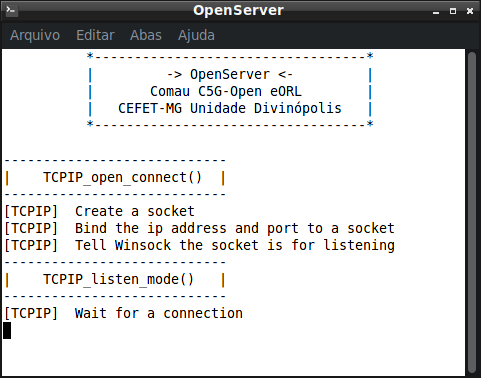
\includegraphics[width=10cm]{imagens/Softwares/openserver-wait_.png}
                \small 
                \centering 
                \caption{OpenServer esperando a conexão de um programa cliente}
                \label{openserver-wait}
            \end{figure}
            
            Quando um cliente se conecta ao servidor é realizada uma troca de pacotes para verificar a integridade da conexão. Caso essa verificação seja bem sucedida o servidor fica esperando o recebimento de instruções do cliente, conforme pode ser visto na Figura~\ref{openserver-ok}. O servidor só atua mediante os comandos do cliente.
            
            \begin{figure}[ht]
                \centering
                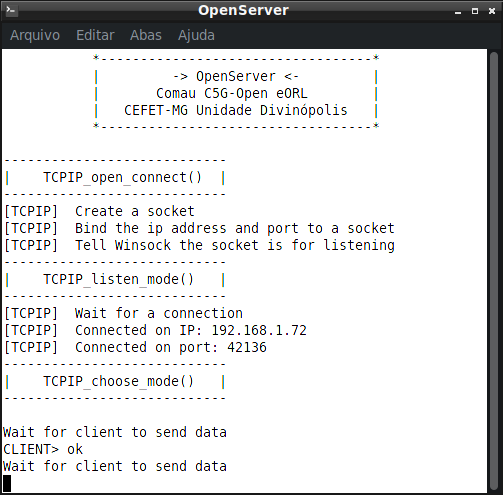
\includegraphics[width=10cm]{imagens/Softwares/openserver-ok_.png}
                \small 
                \centering 
                \caption{OpenServer esperando a instrução do programa cliente conectado}
                \label{openserver-ok}
            \end{figure}
            
            O primeiro caractere recebido pelo servidor informa qual procedimento ele deve seguir. No caso, a instrução `p' é atualmente a instrução padrão, ela está configurada para logo após virem os valores de referência das juntas do robô (truncado em 5 casas decimais, mas, sem uso da vírgula para representar as casas decimais) concatenados na forma de \textit{strings}, como pode ser visto na Figura~\ref{openserver-send}. Ao receber essa instrução, imediatamente o servidor atualiza as variáveis de referência das juntas do robô na memória do programa, que através da \ac{eORL} são enviadas para a controladora. Em seguida, também na forma concatenada sem uso de virgula, o servidor envia a resposta ao programa cliente com a leitura mais recente dos sensores das juntas do robô armazenada na memória do servidor, as quais foram recebidas da controladora.
            
            \begin{figure}[ht]
                \centering
                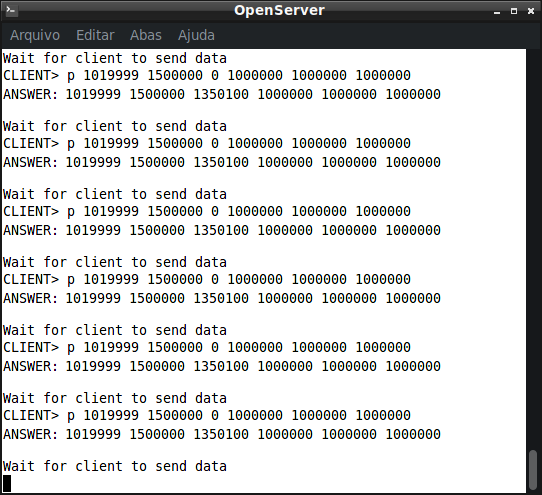
\includegraphics[width=10cm]{imagens/Softwares/openserver-send_.png}
                \small 
                \centering 
                \caption{OpenServer executando a instrução do programa cliente e respondendo com a leitura dos sensores}
                \label{openserver-send}
            \end{figure}
            
            Esta forma de transmitir os dados (\textit{strings} concatenadas) foi desenvolvida com a intenção de ser uma construção simples de ser implementada em outras linguagens de programação.
            
            Para ilustrar o funcionamento em simultâneo do OpenServer, programa cliente e controladora, bem como a comunicação entre eles, foi desenvolvido um fluxograma contendo o funcionamento desta estrutura. O mesmo pode ser visualizado na Figura~\ref{fig:fluxograma}, onde as setas na cor preta mostram o fluxo de funções do programa; as setas na cor ciano indicam a comunicação \textit{Ethernet} entre o dispositivo do cliente e o \ac{LPC}; e as setas na cor magenta indicam a comunicação do \textit{OpenServer} com a controladora do robô.
            
            \begin{figure}[ht]
                \centering
                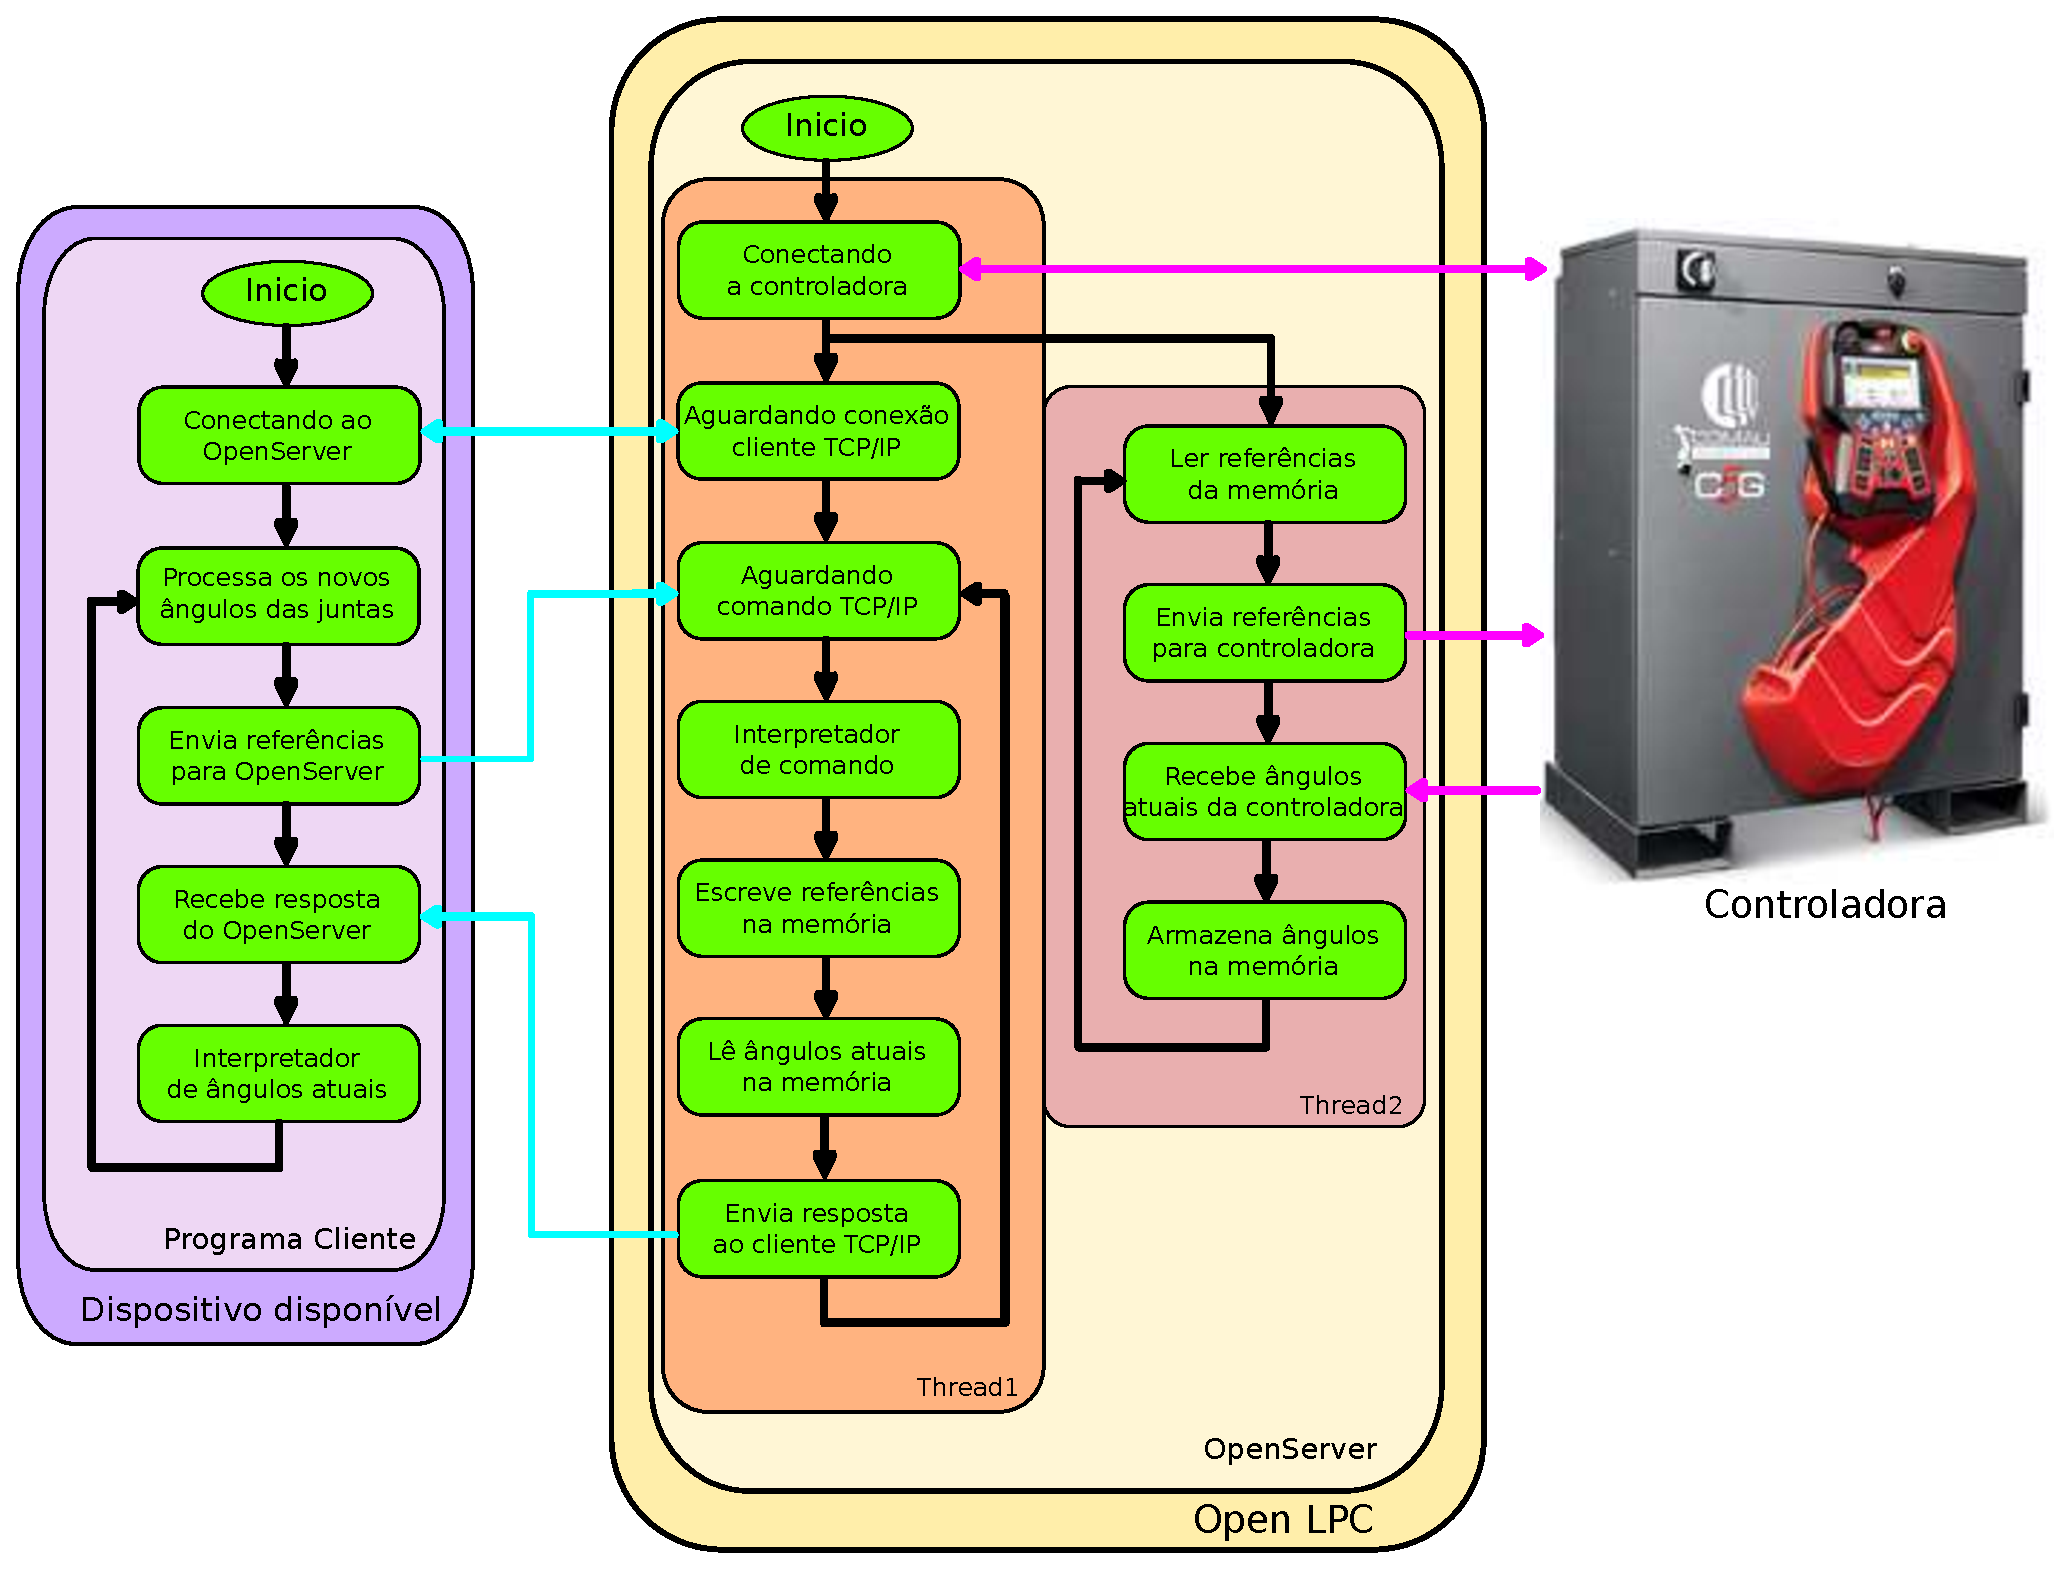
\includegraphics[width=\columnwidth]{imagens/Softwares/infografico.eps}
                \small 
                \centering 
                \caption{Fluxograma do funcionamento e comunicação do OpenServer, programa cliente e controladora.}
                \label{fig:fluxograma}
            \end{figure}
            
            Para executar o OpenServer é pre-requisito a controladora estar ligada e devidamente conectada ao \ac{LPC}, pois a primeira ação que o \textit{OpenServer} faz, quando é iniciado, é se conectar à controladora, como pode ser visto no Fluxograma~\ref{fig:fluxograma}. Caso a conexão não seja bem sucedida o programa é encerrado e, caso seja bem sucedida, o OpenServer abre a possibilidade de um programa cliente se conectar à controladora. Depois de algum cliente se conectar, o OpenServer fica aguardando comandos do programa cliente, sendo os comandos nos formatos explicados anteriormente. Ao receber um comando ele é enviado ao interpretador de comandos que irá extrair os dados de referências das juntas do robô e salvar na memória, por meio da Thread 1. Em seguida, a Thread 1 do OpenServer irá ler da memória os valores atuais de tais ângulos e enviá-los ao programa cliente.
            
            O programa cliente por sua vez é bem mais simples. Depois de se conectar ao \textit{}{OpenServer} ele basicamente executa um loop onde calcula qual a nova POSE do robô, envia para o mesmo as referências de ângulos de juntas via o protocolo \ac{TCPIP} desenvolvido, recebe as referências de ângulos atuais pelo protocolo, interpreta o protocolo para extrair a informação de cada ângulo e então o processo é reiniciado. O funcionamento do programa cliente pode ser adaptado pelo desenvolvedor conforme for atender melhor as suas necessidades.
            
            A controladora aparece no fluxograma como uma caixa preta, ou seja, não se sabe de fato como é implementada a programação da controladora devido ao seu código ser fechado, proprietário da Comau. Algumas informações básicas são disponibilizadas pelo manual e estão fundamentadas no Capítulo~\ref{chp:Fundamentos}.
            
        \subsection{Solução do Problema da Assincronia das Comunicações}
        
            As taxas de transmissão de dados podem não ser necessariamente as mesmas. A taxa de comunicação da \ac{eORL} com a controladora deve ser configurada para ocorrer a uma taxa fixa de \SI{0,4}{\milli\second}, \SI{2}{\milli\second}, \SI{4}{\milli\second}, \SI{8}{\milli\second} ou \SI{16}{\milli\second}, já a taxa de comunicação entre o programa servidor e o programa cliente não tem taxas fixas definidas, podendo inclusive a comunicação ser realizada de forma não constante, sendo o programa cliente responsável por decidir quando enviar um pacote de dados, onde o OpenServer passivamente irá responder imediatamente com outro pacote de dados e voltar a aguardar o recebimento de um novo pacote. Assim o desenvolvedor do programa cliente não tem a responsabilidade de programar o cliente para garantir uma taxa de amostragem fixa, nem do processamento do programa cliente demorar o suficiente para ultrapassar alguma taxa de amostragem pré-definida.
            
            No OpenServer a comunicação com a controladora através da \ac{eORL} ocorre em uma thread separada da comunicação com o programa cliente através do protocolo \ac{TCPIP}. Logo, quando uma instrução em uma thread tentar escrever em uma variável isto pode ocasionar um conflito caso uma instrução em outra thread tente ler a variável ao mesmo tempo. Os algorítimos de comunicação foram implementados de forma a superar esse problema ocasionado pela falta de sincronismo das threads e da comunicação na direção LPC para a C5G e na direção oposta.
            
            O pacote de dados sensoriais das juntas do robô (oriundos da controladora) é armazenado em um ponteiro inteligente local, sobrescrevendo o anterior a medida que vai sendo recebido, e o mesmo é feito com pacote de dados das referências juntas do robô (oriundos do cliente), mas em outro ponteiro inteligente local na outra thread. Quando o pacote de dados acaba de ser transferido para o ponteiro local, imediatamente é dado a instrução do objeto do ponteiro inteligente local ser atribuído a um ponteiro inteligente global, já criado no início na execução do programa. Um ponteiro local para leitura de dados é criado localmente na thread recebendo o objeto do ponteiro global. Desta forma os ponteiros inteligentes globais atuam como uma ponte de comunicação entre os ponteiros locais, permitindo assim que a thread de comunicação \ac{TCPIP} esteja parada em modo listen do \ac{TCPIP}, ou seja, sem atualizar/ler os valores dos ponteiros globais, enquanto a thread de comunicação da controladora do robô esteja trabalhando a uma taxa fixa atualizando e lendo valores nos ponteiros inteligentes globais.
            
            A Figura~\ref{fig:ponteiros} ilustra melhor o funcionamento dos ponteiros inteligentes, onde a letra 'P' se refere a 'ponteiro', 'r' se refere a 'referência' da junta do robô, 's' se refere aos 'sensores' das juntas do robô, '1' e '2' se referem às threads e, por fim, 'g' se refere aos ponteiros 'globais'.
            
            \begin{figure}[H]
                \centering
                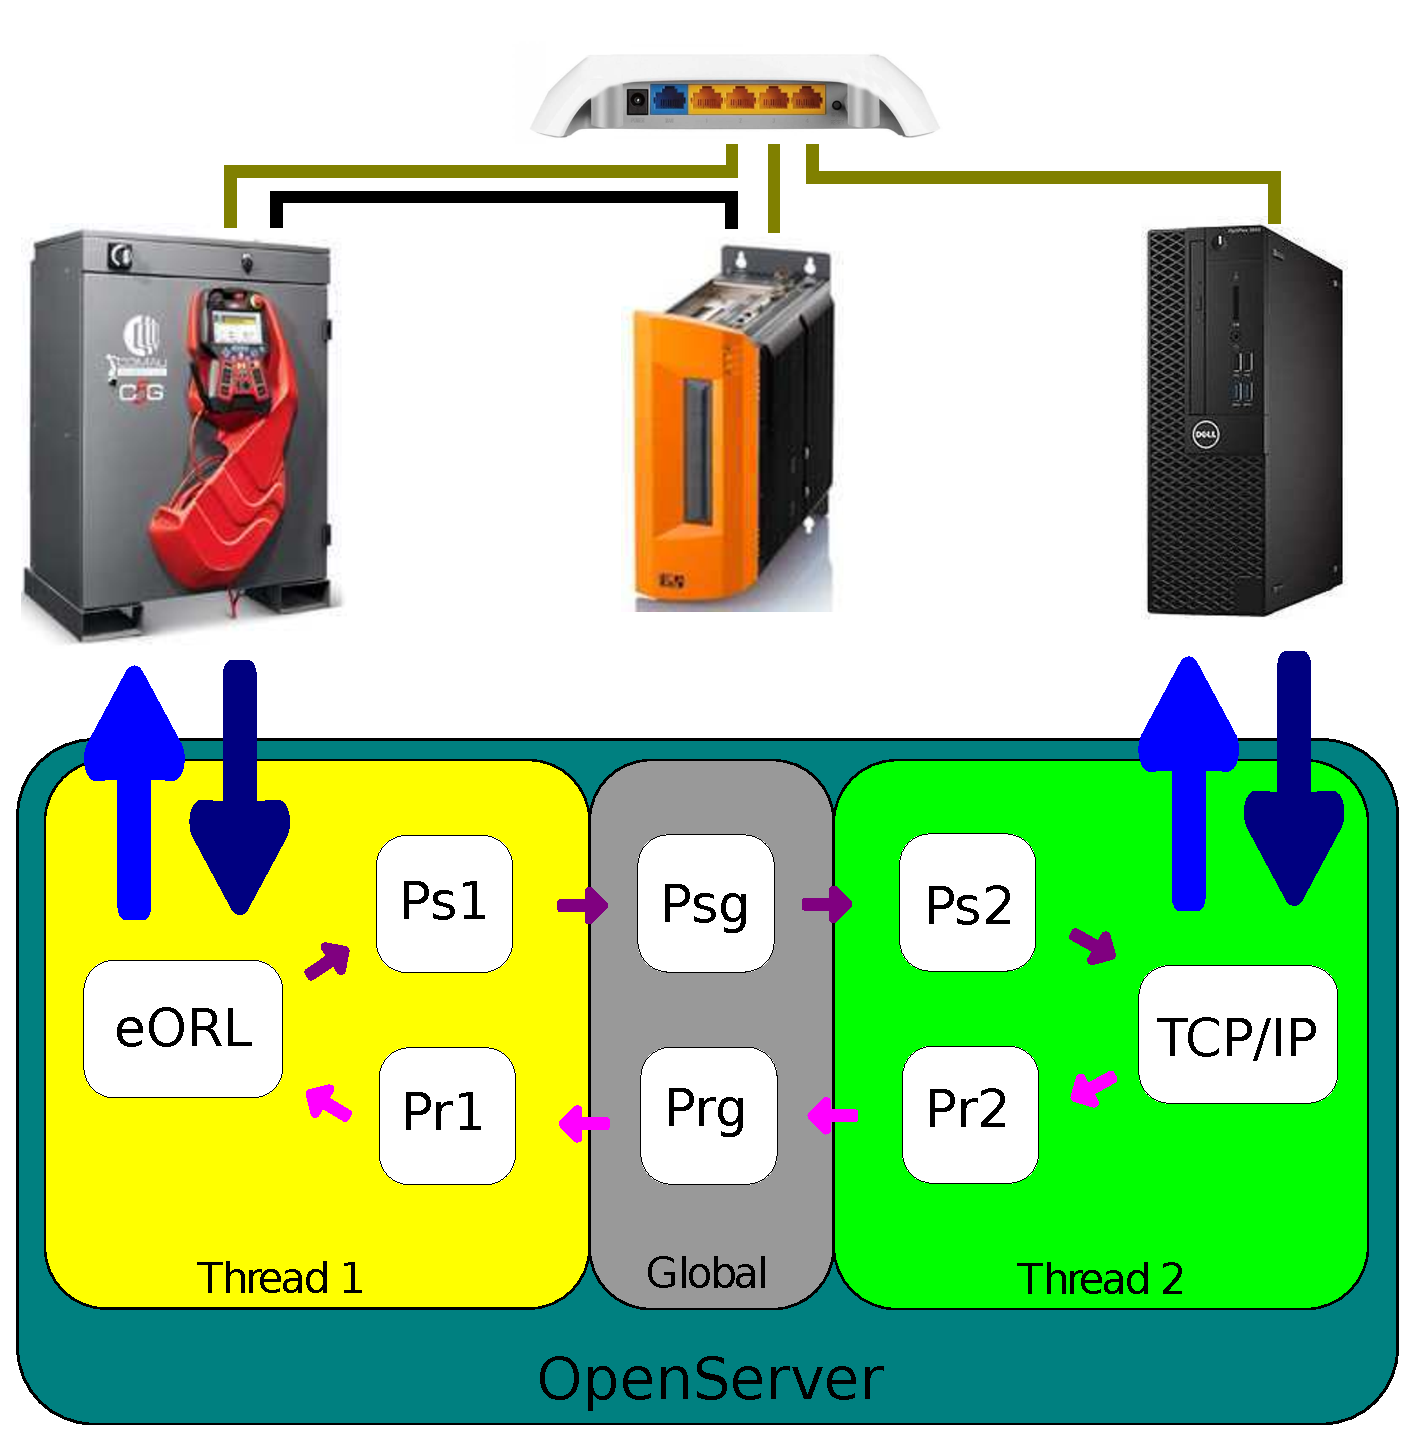
\includegraphics[width=10cm]{imagens/Softwares/ponteiro.eps}
                \small 
                \centering 
                \caption{Funcionamento dos ponteiros inteligentes no OpenServer}
                \label{fig:ponteiros}
            \end{figure}
        
            Desta forma, enquanto a thread de comunicação com o cliente não atualiza na variável global os valores de referência das juntas do robô, a thread de comunicação com a controladora envia repetidamente a última referência salva. Quando a thread de comunicação com o cliente for ler os dados sensoriais da junta do robô no ponteiro global, ela irá ler o pacote de dados mais recente, pois a thread de comunicação com a controladora está continuamente atualizando o pacote de dados em tal ponteiro.
            
            Essa abordagem soluciona o problema da assincronia de comunicação, pois quando ocorre a tentativa de atribuição de um objeto de um ponteiro inteligente local em um global em uma thread, ao mesmo tempo que acontece a tentativa de atribuição de uma ponteiro inteligente global em um local por outra thread, o ponteiro inteligente tem um mecanismo de gerenciamento para tal situação. Ele cria um segundo objeto para ser atribuído enquanto o primeiro é lido. Depois, o primeiro é automaticamente destruído e o segundo objeto passa a ocupar o lugar do primeiro.
        
    \section{O OpenClientExemple}
    
        Para testar o OpenSever foi preciso desenvolver um programa cliente que se comunique com ele via rede \ac{TCPIP}. Este programa foi chamado de \textit{OpenClientExemple}, isto é, um exemplo de cliente do OpenServer. Ele foi escrito em C++ usando bibliotecas padrão para sistemas operacionais baseados em Linux e permite o usuário enviar os ângulos de referência de cada junta do robô e visualizar as leituras dos sensores de posição angular (\textit{encoder} absoluto de precisão) de cada junta em tempo real através de uma interface gráfica que pode ser vista na Figura~\ref{openclient_}. 
    
        \begin{figure}[H]
            \centering
            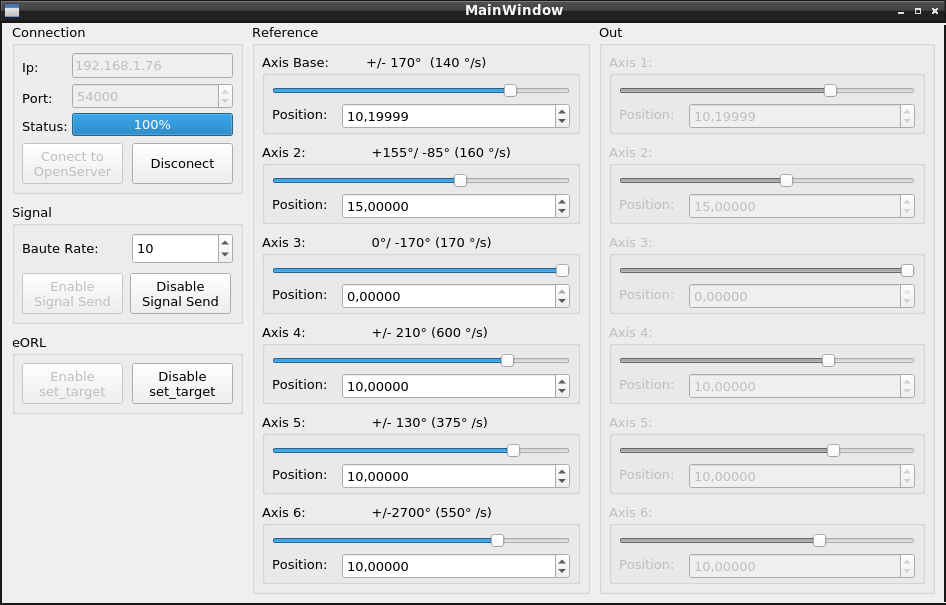
\includegraphics[width=\columnwidth]{imagens/Softwares/openclient_.png}
            \small 
            \centering 
            \caption{Interface gráfica do \textit{OpenClientExemple}}
            \label{openclient_}
        \end{figure}
        
        O funcionamento dele é simplesmente, depois de iniciar a conexão com o OpenServer, ler os valores dos componentes da interface gráfica e enviar para o OpenServer, ao mesmo tempo que recebe os ângulos das juntas vindos do OpenServer e os atualiza nos componentes da interface gráfica.
        